\documentclass[12pt]{article}

\usepackage[margin=1in]{geometry}
\usepackage{amsmath,amssymb,amsfonts,amsthm}
\usepackage{color}
\usepackage{hyperref}
\usepackage{graphicx}
\usepackage{bm}
\usepackage{tikz}
\usetikzlibrary{matrix,arrows,calc,decorations.pathmorphing}

%--------------------------------------------------------------------------------
% Title and Author
%--------------------------------------------------------------------------------
\title{\textbf{A Functorial Approach to Quantum Information and Computation:\\
A Compositional Pipeline from User to Storage}}
\author{
  Matthew Long \\
  \textit{Magneton Labs}
}
\date{\today}

%--------------------------------------------------------------------------------
% Theorem Styles
%--------------------------------------------------------------------------------
\newtheorem{theorem}{Theorem}[section]
\newtheorem{lemma}[theorem]{Lemma}
\newtheorem{definition}[theorem]{Definition}
\newtheorem{proposition}[theorem]{Proposition}
\newtheorem{remark}[theorem]{Remark}
\newtheorem{corollary}[theorem]{Corollary}
\newtheorem{example}[theorem]{Example}

%--------------------------------------------------------------------------------
% Document
%--------------------------------------------------------------------------------
\begin{document}
\maketitle

\begin{abstract}
We present a mathematically rich, functorial framework for describing and analyzing a quantum information pipeline:
\[
\text{User} \;\longrightarrow\; \text{Network} \;\longrightarrow\; \text{Computation} \;\longrightarrow\; \text{Database} \;\longrightarrow\; \text{Storage}.
\]
Each stage is formulated as a functor that preserves and transforms the structure of quantum information, encapsulating superposition, entanglement, error correction, and measurement dynamics. We discuss how the composite functor yields an end-to-end mapping of quantum data from user input to long-term storage, providing a powerful language for modular design, implementation details, and rigorous correctness proofs. Additionally, we propose a multi-phase timeline for realizing this pipeline in practical quantum computing architectures. 
\end{abstract}

\tableofcontents

\section{Introduction}

The development of quantum information science has prompted a re-examination of many classical concepts in communication, computation, and data storage. In the classical domain, we naturally describe information pipelines---user input, communication networks, computational engines, databases, and long-term storage---as interconnected layers. Within quantum settings, such layered systems become more intricate due to quantum effects such as superposition, entanglement, and the collapse of states upon measurement.

Category theory, and in particular the language of \textit{functors}, provides a unifying viewpoint for describing these systems. By capturing the relationships between structures (objects) and processes (morphisms), we can describe the passage of quantum information as a composition of functors between suitable categories. This \textit{functorial} approach clarifies how each layer behaves on quantum states, preserving their delicate properties where required (e.g., entanglement) and accounting for interactions with classical infrastructure.

This paper sets out to formalize such a functorial framework:

\begin{itemize}
\item We introduce the abstract categories needed to represent quantum states, quantum operations, and the interface with classical data.
\item We show how each stage of a quantum pipeline can be represented as a functor, focusing on how each functor preserves or transforms the structure of the quantum data.
\item We then compose these functors to form an end-to-end map from ``User'' objects (quantum or classical input) to ``Storage'' objects (physical quantum registers, fault-tolerant memory, etc.).
\item We conclude by proposing a timeline that delineates incremental steps toward practical implementation of these ideas, given current quantum hardware and theoretical constraints.
\end{itemize}

Throughout, we strive to make the mathematics concrete enough for real-world applications, yet sufficiently general to encompass a broad range of quantum computational architectures.

\section{Preliminaries}

This section provides a brief review of the mathematical concepts that we will use throughout the paper.

\subsection{Categories, Functors, and Natural Transformations}

\begin{definition}[Category]
A \emph{category} $\mathcal{C}$ consists of:
\begin{itemize}
\item A class of \emph{objects}, denoted by $\mathrm{Ob}(\mathcal{C})$.
\item For each pair of objects $A, B \in \mathrm{Ob}(\mathcal{C})$, a set $\mathrm{Hom}(A,B)$ of \emph{morphisms} (or \emph{arrows}) from $A$ to $B$.
\item A composition law that takes a morphism $f \in \mathrm{Hom}(A,B)$ and $g \in \mathrm{Hom}(B,C)$ to produce a morphism $g \circ f \in \mathrm{Hom}(A,C)$.
\item An identity morphism $\mathrm{id}_A \in \mathrm{Hom}(A,A)$ for each object $A$.
\end{itemize}
This structure is subject to the usual associativity and identity axioms.
\end{definition}

\begin{definition}[Functor]
A \emph{functor} $F: \mathcal{C} \to \mathcal{D}$ between two categories $\mathcal{C}$ and $\mathcal{D}$ is a mapping that:
\begin{itemize}
\item Assigns to each object $A \in \mathrm{Ob}(\mathcal{C})$ an object $F(A) \in \mathrm{Ob}(\mathcal{D})$.
\item Assigns to each morphism $f: A \to B$ in $\mathcal{C}$ a morphism $F(f): F(A) \to F(B)$ in $\mathcal{D}$.
\end{itemize}
Such that $F(\mathrm{id}_A) = \mathrm{id}_{F(A)}$ and $F(g \circ f) = F(g) \circ F(f)$.
\end{definition}

\begin{definition}[Natural Transformation]
A \emph{natural transformation} $\eta: F \Rightarrow G$ between two functors $F, G: \mathcal{C} \to \mathcal{D}$ assigns to each object $A \in \mathcal{C}$ a morphism $\eta_A: F(A) \to G(A)$ in $\mathcal{D}$ such that for every morphism $f: A \to B$ in $\mathcal{C}$, the following diagram commutes:

\[
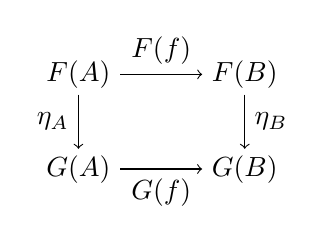
\begin{tikzpicture}[baseline=(current bounding box.center)]
  \matrix(m)[matrix of math nodes, row sep=2em, column sep=3em,
    text height=1.5ex, text depth=0.25ex]
  {
    F(A) & F(B) \\
    G(A) & G(B) \\
  };
  \path[->]
    (m-1-1) edge node[above]{$F(f)$} (m-1-2)
    (m-1-1) edge node[left]{$\eta_A$} (m-2-1)
    (m-1-2) edge node[right]{$\eta_B$} (m-2-2)
    (m-2-1) edge node[below]{$G(f)$} (m-2-2);
\end{tikzpicture}
\]
\end{definition}

\subsection{Quantum Mechanics in Categorical Terms}

At the heart of quantum information theory, we have:
\begin{itemize}
\item \textbf{Hilbert Spaces} as objects.
\item \textbf{Linear Maps (Unitary, Completely Positive Maps)} as morphisms.
\end{itemize}

For quantum information and computation, we often consider the category:
\[
\mathbf{FHilb}
\]
whose objects are finite-dimensional Hilbert spaces over $\mathbb{C}$ (e.g., $\mathbb{C}^2$ for qubits) and whose morphisms are linear maps.

However, to capture the full breadth of quantum processes (which include measurements, partial traces, etc.), one often studies the category of completely positive maps or \emph{superoperators}, or uses $\mathbf{CPM}(\mathbf{FHilb})$ in which objects are Hilbert spaces and morphisms are completely positive trace-preserving (CPTP) maps.

\subsection{The Compositional Pipeline Idea}

We are considering a compositional pipeline:
\[
\text{User} \;\longrightarrow\; \text{Network} \;\longrightarrow\; 
\text{Computation} \;\longrightarrow\; \text{Database} \;\longrightarrow\; 
\text{Storage}.
\]
Each arrow is interpreted as a functor that preserves the relevant structures of quantum data, such as coherence, entanglement, and error correction codes.

In classical data systems, these are often discrete steps. In quantum systems, each step must preserve the linear structure of the states, carefully manage noise, and (in many cases) handle the interplay between quantum and classical data (e.g., measurement outcomes stored classically that then influence future quantum operations).

\section{A Category-Theoretic Model of a Quantum Pipeline}

We now formalize the pipeline using categories and functors.

\subsection{Stage 1: User to Network}

\begin{definition}[User Category, $\mathcal{U}$]
We define $\mathcal{U}$ to be the category capturing user interactions or \emph{inputs}. Depending on context, objects in $\mathcal{U}$ can be:
\begin{itemize}
\item Classical input states (e.g., strings of bits).
\item Quantum states prepared by the user (e.g., specific qubit states).
\end{itemize}
Morphisms in $\mathcal{U}$ might describe transformations of user intentions or re-encodings of initial data.
\end{definition}

\begin{definition}[Network Category, $\mathcal{N}$]
We let $\mathcal{N}$ represent the category of networked transmission protocols. Its objects are quantum or classical states \emph{in transit}, and morphisms are physical processes that send these states from one location to another (quantum channels, classical channels, or hybrid channels).
\end{definition}

\begin{definition}[Network Functor, $F: \mathcal{U} \to \mathcal{N}$]
The functor $F$ maps a user input object $U \in \mathrm{Ob}(\mathcal{U})$ to a corresponding network transmission object $F(U)$, representing that data en route. It also maps morphisms in $\mathcal{U}$ (re-encodings, user transformations) to morphisms in $\mathcal{N}$ (appropriate transmissions with error correction).
\end{definition}

Concretely, if the user’s input is a qubit state $\vert \psi \rangle \in \mathcal{H}_2$, the functor $F$ might encode that state into a quantum error correction code, then pass it through a noisy quantum channel that is recognized as a morphism in $\mathcal{N}$. The key point is the \textit{functorial} requirement that $F$ must preserve composition and identities, ensuring coherence of user transformations at the network layer.

\subsection{Stage 2: Network to Computation}

\begin{definition}[Computation Category, $\mathcal{C}$]
We define $\mathcal{C}$ to be the category capturing the quantum (and possibly classical) computations performed on the transmitted data. Objects are typically Hilbert spaces representing the system states post-transmission; morphisms may be unitary operators, CPTP maps, or measurement processes (often expressed as an isomorphism to $\mathbf{CPM}(\mathbf{FHilb})$).
\end{definition}

\begin{definition}[Computation Functor, $G: \mathcal{N} \to \mathcal{C}$]
The functor $G$ takes network-level states to computational states and channels to the actual computational routines. For instance, if $F(U)$ is in an encoded form, $G(F(U))$ might be the decoded form inside a quantum processor where unitaries or gates are applied.
\end{definition}

Again, the functorial viewpoint forces consistency: composition of network-level protocols followed by standard computational gates should match a single, well-defined morphism in $\mathcal{C}$.

\subsection{Stage 3: Computation to Database}

\begin{definition}[Database Category, $\mathcal{D}$]
We let $\mathcal{D}$ represent the organization of processed data. Objects in $\mathcal{D}$ could be quantum states structured as records, or more exotic structures capturing entanglement across many qubits. Morphisms represent queries, transformations of data schema, or partial measurements used for indexing.
\end{definition}

\begin{definition}[Database Functor, $H: \mathcal{C} \to \mathcal{D}$]
The functor $H$ maps a computational state to an organized quantum data structure. For instance, if the computation produces multiple entangled states, $H$ would map each to a separate \emph{entry} in the quantum database, preserving entanglement correlations or storing them in error-corrected registers as required.
\end{definition}

The role of $H$ is crucial in bridging \emph{dynamic} quantum computation and \emph{static} (or semi-static) quantum data organization. It must handle the partial measurement that might be required to create classical indexes without destroying all quantum correlations.

\subsection{Stage 4: Database to Storage}

\begin{definition}[Storage Category, $\mathcal{S}$]
We define $\mathcal{S}$ as the category whose objects are physical quantum memory devices (e.g., arrays of trapped ions, superconducting qubits, topological qubits) and whose morphisms are processes that store, retrieve, or move these states in a physical substrate.
\end{definition}

\begin{definition}[Storage Functor, $I: \mathcal{D} \to \mathcal{S}$]
The functor $I$ maps the quantum (and possibly classical) records in the database to physical memory. Morphisms correspond to storage or retrieval operations that preserve the quantum coherence or maintain error-correcting codes.
\end{definition}

When we \emph{compose} all these functors, we obtain:
\[
I \circ H \circ G \circ F: \quad \mathcal{U} \;\longrightarrow\; \mathcal{S}.
\]
This composite is a \emph{homomorphism} that preserves the structure at each intermediate stage, ensuring an end-to-end translation of user data into stored quantum states.

\section{Ensuring Quantum Integrity: Error Correction in the Functorial Framework}

A major challenge is how quantum error correction (QEC) fits into this pipeline. Functorially, QEC can appear in multiple stages:
\begin{itemize}
\item \emph{Network-level} error correction to handle noise in transmission.
\item \emph{Computation-level} error correction to maintain coherence across gate operations.
\item \emph{Database-level} error correction that ensures data integrity for long-lived states.
\item \emph{Storage-level} error correction to mitigate decoherence in memory.
\end{itemize}

\subsection{Logical vs. Physical Qubits}
We can refine the categories at each stage to distinguish between \emph{physical} and \emph{logical} qubits:

\[
\mathcal{N}_{\mathrm{phys}} \xrightarrow{\;\;QEC\;\;} \mathcal{N}_{\mathrm{log}}, 
\quad
\mathcal{C}_{\mathrm{phys}} \xrightarrow{\;\;QEC\;\;} \mathcal{C}_{\mathrm{log}},
\quad
\ldots
\]
A QEC scheme is itself a functor $E:\mathcal{X}_{\mathrm{phys}} \to \mathcal{X}_{\mathrm{log}}$ (where $\mathcal{X}$ could be $\mathcal{N}$, $\mathcal{C}$, or $\mathcal{D}$). This functor preserves the quantum information content but typically inflates the dimension (encoding one logical qubit into many physical qubits).

\subsection{Composing QEC with the Main Pipeline}

One may compose the main pipeline functors with error-correcting functors in such a way that the entire pipeline remains consistent. For instance, at the \emph{network} stage, we might have:
\[
F_{\mathrm{phys}}: \mathcal{U} \to \mathcal{N}_{\mathrm{phys}}, 
\quad
E_{\mathrm{net}}: \mathcal{N}_{\mathrm{phys}} \to \mathcal{N}_{\mathrm{log}},
\quad
G: \mathcal{N}_{\mathrm{log}} \to \mathcal{C}_{\mathrm{log}}.
\]
Thus, the composition $G \circ E_{\mathrm{net}} \circ F_{\mathrm{phys}}$ provides a robust route from user input to the computational regime with error correction accounted for.

\section{Measurement and Classical Data Interactions}

\subsection{Measurement as a Non-Functorial Operation?}
A common concern is that measurement seemingly breaks the linear structure central to quantum theory, as measurement is inherently a \emph{non-unitary}, \emph{probabilistic} process. Categorical quantum mechanics addresses this by expanding the concept of morphisms to encompass more general \emph{completely positive} maps. Measurement can be seen as a special case of a quantum channel, which, upon composition, yields classical outputs.

\subsection{Enriching the Categories with Classical Data}
In practice, many quantum protocols require feed-forward classical information (e.g., measurement outcomes that determine subsequent gates). This calls for an enriched or braided structure, sometimes referred to as $\mathbf{C^*}$-categories or using the notion of \emph{dagger compact categories}. The upshot is that we can incorporate classical control flows as objects or morphisms in an augmented category and treat quantum-classical interplay functorially.

\section{Implementation Timeline}

Realizing an end-to-end quantum pipeline in practice requires iterative development across hardware, software, and theoretical frameworks. Below is a proposed multi-phase timeline:

\subsection*{Phase I: Foundational Infrastructure (1--2 years)}
\begin{enumerate}
\item \textbf{Hybrid Networks}: Implement partial quantum networks that can reliably transport qubits short distances with moderate fidelity (e.g., local fiber links or integrated superconducting platforms).
\item \textbf{Minimal QEC Integration}: Demonstrate small-scale quantum error correction (e.g., surface codes with a handful of physical qubits).
\item \textbf{Functorial Prototypes}: Develop small prototypes in research labs to show that the mapping from user-prepared states to network-level states (the $F$ functor) and from network-level states to basic computations ($G$) preserves structure in a toy model (e.g., 2--3 qubits).
\end{enumerate}

\subsection*{Phase II: Intermediate Scale (3--5 years)}
\begin{enumerate}
\item \textbf{Reliable Computation Nodes}: Scale quantum processors to tens or hundreds of logical qubits, enabling more complex unitaries.
\item \textbf{Database Prototypes}: Create small quantum databases ($H$ functor) storing entangled states with partial measurement queries to illustrate how data structures in $\mathcal{D}$ can be physically instantiated.
\item \textbf{Storage Hardware}: Begin employing stable physical media (trapped ions, superconducting circuits with long coherence times, or topological qubits) for quantum memory ($I$ functor).
\end{enumerate}

\subsection*{Phase III: Fault-Tolerant Systems (5--10 years)}
\begin{enumerate}
\item \textbf{Global Quantum Networks}: Establish reliable quantum repeaters and entangled nodes to handle longer-distance quantum communications.
\item \textbf{Fully Functorial Pipeline}: Integrate error correction at each stage and demonstrate an end-to-end pipeline with robust composition $I \circ H \circ G \circ F$ for practical problem sizes.
\item \textbf{Hybrid Classical-Quantum Databases}: Develop advanced quantum database systems that share data with classical infrastructure while preserving quantum advantages (e.g., secure multi-party queries).
\end{enumerate}

\subsection*{Phase IV: Large-Scale Integration (10+ years)}
\begin{enumerate}
\item \textbf{Industry Integration}: Incorporate large quantum databases into mainstream cloud services, allowing user queries and computations to interface seamlessly with quantum back-ends.
\item \textbf{Refined Categorical Frameworks}: Evolve the theoretical foundations to account for large-scale entanglement, advanced error correction, and resource management. Possibly exploit new forms of topological quantum computation or beyond.
\item \textbf{Standards and Interoperability}: Standardize the functorial frameworks for quantum platforms, ensuring \emph{plug-and-play} modules at each pipeline stage.
\end{enumerate}

\section{Discussion and Outlook}

A functorial viewpoint on quantum information pipelines has several advantages:

\begin{enumerate}
\item \textbf{Modularity}: By formalizing each stage as a functor, we can replace or upgrade a specific stage (e.g., new QEC code for the network) while preserving the overall structure of the pipeline.
\item \textbf{Compositional Correctness}: Functorial composition imposes consistency. If the pipeline is correct in parts, it is correct as a whole, subject to well-defined morphisms.
\item \textbf{Abstraction vs. Realism}: Category theory provides high-level abstractions, but the relevant categories must still reflect physical realities like decoherence, noise, and finite resources. The interplay between abstract design and concrete hardware constraints is bridged by carefully constructing the categories and functors.
\item \textbf{Multi-Disciplinary Integration}: The pipeline perspective helps unify physics (quantum states), computer science (data structures, algorithms), and engineering (networks, hardware) under one mathematical umbrella.
\end{enumerate}

\section{Conclusion}

In this paper, we have outlined a functorial approach to quantum information flow through an end-to-end pipeline:
\[
\text{User} \;\longrightarrow\; \text{Network} 
\;\longrightarrow\; \text{Computation} 
\;\longrightarrow\; \text{Database} 
\;\longrightarrow\; \text{Storage}.
\]
By regarding each intermediate stage as a functor, we ensure that the structure of quantum information is preserved wherever possible, and that the necessary transitions (error correction, partial measurement, encoding/decoding) are rigorously accounted for in a composite mapping. 

We also provided a roadmap for implementing such a pipeline, noting incremental improvements in quantum hardware, network infrastructure, and database technologies that would be necessary. This functorial vision is still in its infancy, but as quantum hardware scales and software components mature, the categorical language may prove invaluable in designing robust, modular, and correct-by-construction quantum systems.

\vspace{1cm}

\noindent \textbf{Acknowledgments.} 
The author acknowledges insightful discussions with colleagues at Magneton Labs and thanks the broader quantum information community for foundational research that inspires compositional frameworks.

\vspace{0.5cm}

%--------------------------------------------------------------------------------
% References
%--------------------------------------------------------------------------------
\begin{thebibliography}{99}

\bibitem{nielsenChuang}
M.~A.~Nielsen and I.~L.~Chuang, 
\textit{Quantum Computation and Quantum Information}, 
Cambridge University Press, 10th Anniversary Ed., 2010.

\bibitem{maclane}
S.~Mac Lane, 
\textit{Categories for the Working Mathematician}, 
Springer, 2nd Ed., 1998.

\bibitem{selingerSurvey}
P.~Selinger, 
``A survey of graphical languages for monoidal categories,''
\textit{New Structures for Physics}, Springer, 2009, pp. 289--355.

\bibitem{abramskyCoecke}
S.~Abramsky and B.~Coecke, 
``A categorical semantics of quantum protocols,''
\textit{Proceedings of the 19th Annual IEEE Symposium on Logic in Computer Science}, 2004, pp.~415--425.

\bibitem{baezStay}
J.~C.~Baez and M.~Stay, 
``Physics, topology, logic and computation: a Rosetta Stone,''
\textit{New Structures for Physics}, Springer, 2010, pp.~95--172. \\
\texttt{arXiv:0903.0340}

\bibitem{gottesman}
D.~Gottesman,
``Stabilizer Codes and Quantum Error Correction,''
\textit{PhD Thesis}, California Institute of Technology, 1997. 
\texttt{arXiv:quant-ph/9705052}

\bibitem{preskill}
J.~Preskill,
``Quantum Computing in the NISQ era and beyond,''
\textit{Quantum} \textbf{2}, 79 (2018).

\end{thebibliography}

\end{document}
